\subsection{Base de données}
Nous allons créer une base de données en utilisant l'exemple de posts sur un blog.


\subsubsection[PHPMyAdmin][]{\phpmyadmin{}}
\phpmyadmin{} est une interface permettant à des ignares comme nou\ldots comme vous* de manipuler et de visualiser le contenu des bases de données facilement sans connaissances en \mysql. Normalement, la configuration a été effectuée lors de la formation précédente et vous devriez pouvoir y accéder en vous rendant sur \url{http://tutolaravel:8080}\footnote{Ou bien \url{http://localhost:8080}, cela dépend de l'url que vous avez choisi dans le \texttt{.env}.}.

\subsubsection[Models][laravel.com/docs/12.x/eloquent\#generating-model-classes]{Models}
Comme dit dans la \texttt{Section~\ref{sec:fonctionnement&philosophie}}, le \model{} \footnote{Rien à voir avec Kendall Jenner, reste concentré sur la formation.} est l'objet qui nous permettra d'interagir avec les \textit{posts} stockés dans notre base de données \footnote{Pour chaque nouvel objet, on aura un \model{} correspondant.}. Pour le créer, tapez \verb|sail artisan make:model Post -m|.
Cela génère un fichier \verb|Post.php|, dans \verb|/app/Models/|.
On peut déjà y ajouter des propriétés comme \verb|$fillable|, qui définissent quels champs peuvent être remplis automatiquement lors de la création d'un nouvel enregistrement
\begin{figure}[H]
  \centering
  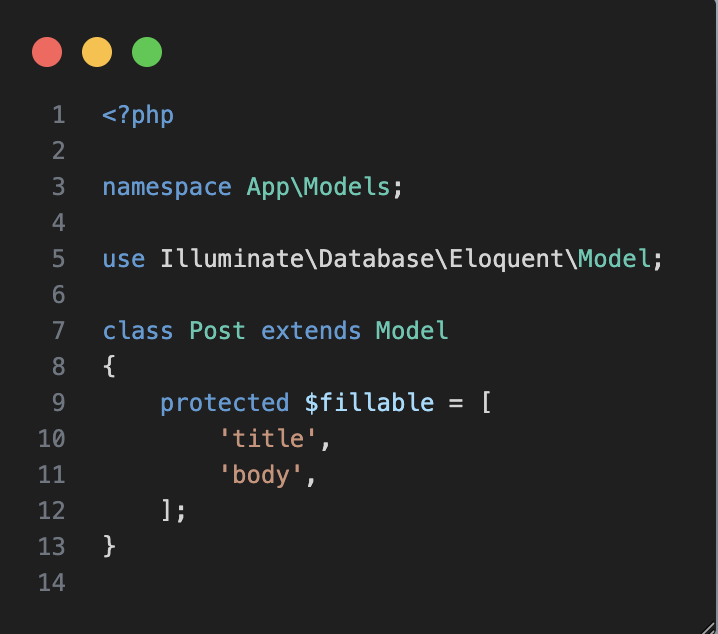
\includegraphics[width=0.2\linewidth]{figures-C1/postmodel.png}
  \caption{Exemple d’un modèle Laravel \texttt{Post}}
\end{figure}
Voici une explication du code:
\begin{itemize}
  \item \verb|namespace App\Models;| : indique dans quel « dossier logique » se trouve notre classe.  
  \item \verb|use Illuminate\Database\Eloquent\Model;| : importe la classe de base \texttt{Model} de Laravel.  
  \item \verb|class Post extends Model| : on crée une classe \texttt{Post} qui hérite de \texttt{Model}, donc qui bénéficie de toutes les fonctionnalités Eloquent.  
  \item \verb|protected $fillable = ['title', 'body'];| : on définit les colonnes de la table qui peuvent être assignées en masse (par exemple avec \verb|Post::create([...])|). Ici, on autorise \texttt{title} et \texttt{body}.  
\end{itemize}
Ainsi, notre model n'est plus un bout de code vide, mais un véritable objet capable de gérer des données venant de la base.

\subsubsection[Migrations: théorie][laravel.com/docs/12.x/migrations\#introduction]{Migrations: comme les oiseaux?}

Une \migration{} est un fichier qui permet de définir les \tables{} de notre base de données. Une \table{} est grosso modo un type de donnée que la \db{} va stocker. Par exemple, la liste de tous les utilisateurs est une \table{}, tout comme les \textit{posts} que nous allons créer. Chaque \table{} contient un certain nombre de \columns{} qui, elles sont les données stockées en tant que telles. En l'occurrence, notre \table{} de \textit{posts} doit contenir une \column{} pour le titre d'un \textit{post} et une pour son contenu en lui-même \footnote{Tous ces termes sont compliqués à décrire avec des mots, mais sont en réalité très intuitifs quand on imagine les données affichées dans un grand tableau à double entrée.}.

Pour créer notre migration, tapez \verb|rien du tout| car la \migration{} a été créée en même temps que notre \model{} grâce au \verb|-m|! Elle se trouve dans \\\verb|database/migration/xxxx_xx_xx_xxxxxx_create_posts_table.php|. \\Ensuite, remplissez-la comme à la \textsc{Figure~\ref{fig:basic_migration}}\footnote{lignes 16 et 17, de rien.}:

Analysons tout a:
\begin{itemize}
    \item \verb|function up()| et \verb|function down()|: La première est exécutée quand on souhaite créer les \tables{} à l'intérieur tandis que la deuxième est exécutée lorsqu'on souhaite supprimer les \tables{} de la \db{}. Pour l'utilisation simple que nous faisons des \migrations{}, pensez à \verb|down| tout ce que vous \verb|up|-per.
    \item \verb|Schema::create('posts',...| en gros, c'est la fonction utilisée pour créer la table \verb|'posts'|, et les \verb|$table->| qui suivent permettent de définir chaque \column{} de la table créée.
    \item \verb|id()|: l'id est ce qu'on appelle la \texttt{Primary Key}. Unique pour chaque \row{}\footnote{une \row{} est un élément de donnée dans une \table{}.}, il permet d'identifier chaque élément de donnée. Il se trouve par défaut sur chaque \table{} nouvellement créée.
    \item \verb|string()| permet de créer une \column{} de type string, de taille 255. La taille est modifiable en ajoutant un nombre <255 en second argument.
    \item \verb|mediumtext()| permet de créer une \column{} de $16.777.215$ charactères (oula).
    \item \verb|timestamps()| ajoute une date de création et de modification à la \table{}. Ces deux \columns{} sont également ajoutées par défaut.
\end{itemize}

\begin{wrapfigure}[17]{r}{0.5\textwidth}
    \vspace{-0.5cm}
    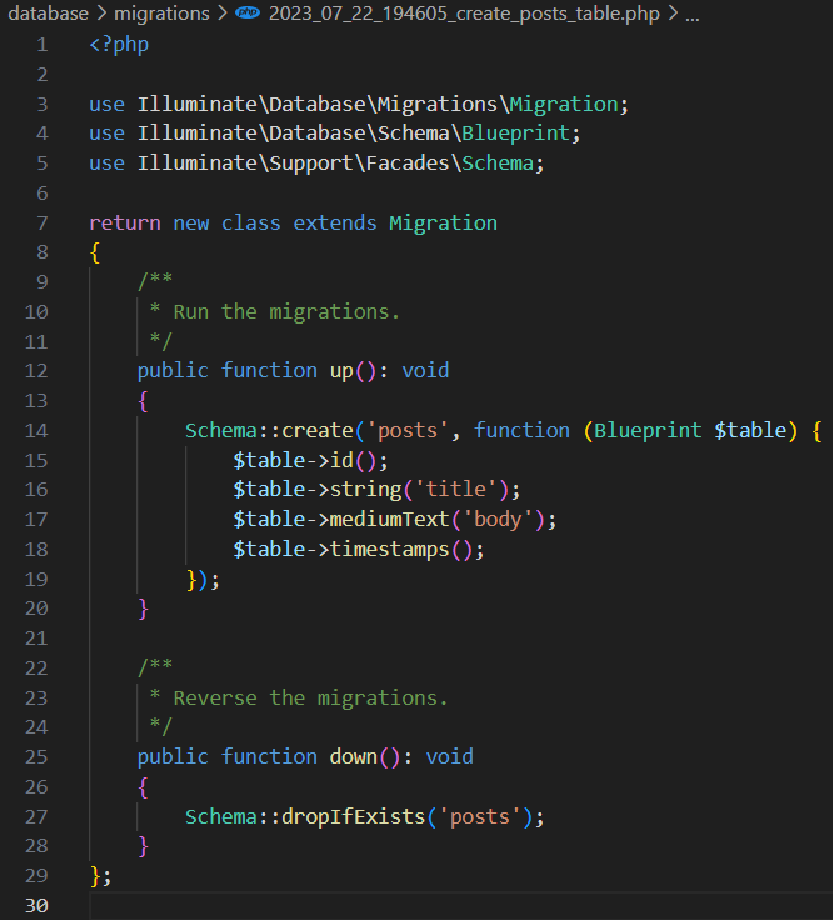
\includegraphics[width=0.5\textwidth]{figures-C1/post_migration.pdf}
    \caption{Exemple très simple de \migration{}\label{fig:basic_migration}}
\end{wrapfigure}
Quelques remarques supplémentaires:

\begin{enumerate}
    \item Par défaut, les \columns{} doivent obligatoirement posséder une valeur.
    \item On peut ajouter de nombreux paramètres aux \columns{} pour modifier leur comportements (exemple: \verb|->nullable()| pour leur permettre d'être vide).
    \item Les types des \column{} correspondent chacune à un type de valeur de \mysql{}, le ``vrai'' langage pour communiquer avec les \db{} duquel \laravel{} nous protège grâce aux \models{}, \migrations{}, \tables{} que nous venons de voir.
\end{enumerate}

Encore une fois, parcourir la doc officielle de \laravel{} permet d'en apprendre beaucoup plus que ce que le tutoriel ne pourra jamais vous apprendre!

\subsubsection[Migrations: exécution]{Migrations: exécution}

Bon, après tant de blabla, passons à l'action. Mais avant cela, \laravel{} nous embête (pour une fois). Afin de n'avoir aucune erreur en exécutant la migration, il va falloir ajouter ces lignes dans \verb|app/Providers/AppServiceProvider.php|:

\begin{figure}[!h]
    \centering
    \begin{minipage}{0.49\textwidth}
         \centering
         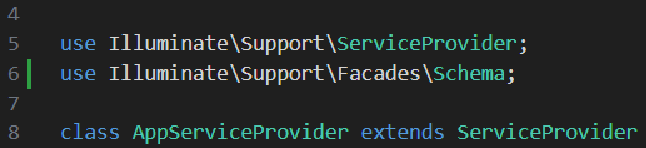
\includegraphics[width=\textwidth]{figures-C1/appservice_2.pdf}
    \end{minipage}
    \begin{minipage}{0.49\textwidth}
         \centering
         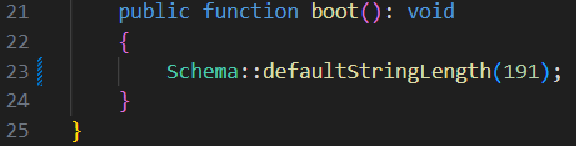
\includegraphics[width=0.95\textwidth]{figures-C1/appservice_1.pdf}
    \end{minipage}
\end{figure}

Voilà! maintenant tapez \verb|sail artisan migrate:fresh --seed| (où \verb|fresh| signifie que tout ce qui existait avant est supprimé et \verb|--seed| permet d'exécuter les \texttt{seeders} vus dans la \texttt{Section~} (WIP)) et, si tout va bien, vous verrez maintenant cela en allant dans \phpmyadmin{}:

\begin{figure}[!h]
    \centering
    \begin{minipage}{0.49\textwidth}
         \centering
         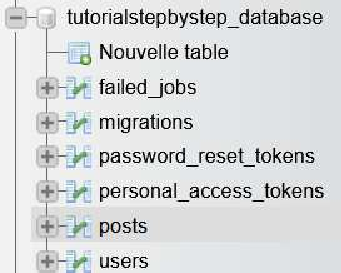
\includegraphics[width=0.6\textwidth]{figures-C1/db_posts_1.pdf}
    \end{minipage}
    \begin{minipage}{0.49\textwidth}
         \centering
         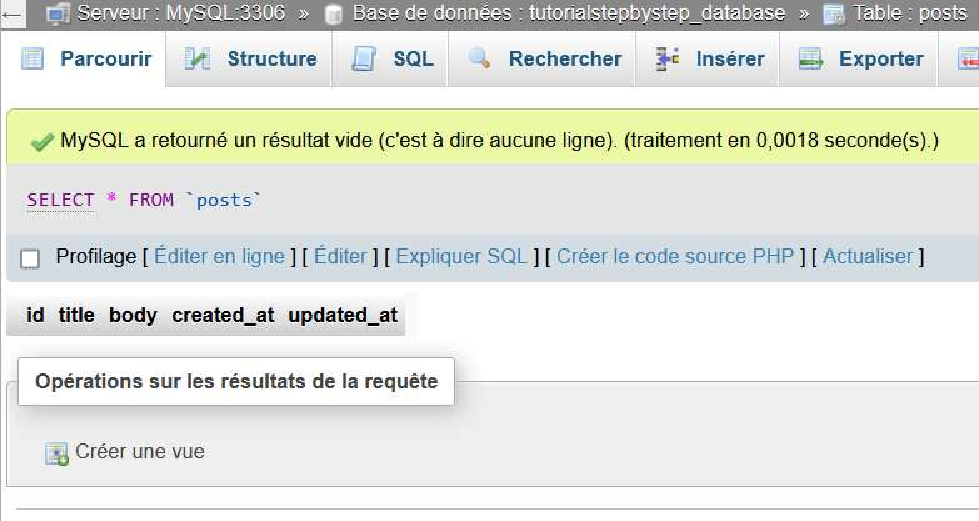
\includegraphics[width=0.9\textwidth]{figures-C1/db_posts_2.pdf}
    \end{minipage}
\end{figure}

\subsubsection[PostsController][laravel.com/docs/12.x/controllers\#resource-controllers]{PostsController}

Pour gérer ces posts, nous allons bien entendu avoir besoin d'un \controller{}. Comme ce genre de données va avoir des manipulations basiques très communes (création, liste, affichage, modification, suppression,\ldots), il existe un certain type de controller permettant de nous faire gagner du temps: le \texttt{resource} \controller{}. Tapez donc \\
\verb|sail artisan make:controller PostsController --resource| pour en créer un.

Ensuite, il faut évidemment définir des nouvelles routes. Une seule ligne toute simple nous permet de générer en réalité 7 \routes{} différentes que nous verrons petit à petit. Ajoutez donc ces 2 lignes dans \verb|routes/web.php|:

\begin{figure}[!h]
    \centering
    \begin{minipage}{0.6\textwidth}
        \centering
        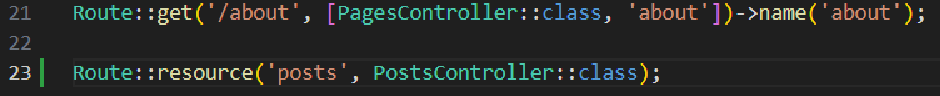
\includegraphics[width=\textwidth]{figures-C1/res_route_1.pdf}
        \caption{\texttt{routes/web.php}}
        \label{fig:post_route}
    \end{minipage}
    \begin{minipage}{0.38\textwidth}
        \centering
        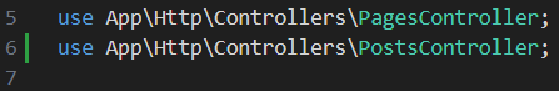
\includegraphics[width=\textwidth]{figures-C1/res_route_2.pdf}
        \caption{}
    \end{minipage}
\end{figure}
\vspace{-0.5cm}
Notez que en donnant \textit{'posts'} en argument à \verb|resource()|, celui-ci fait automatiquement lien avec le \model{} \verb|Post|\footnote{Pour comprendre comment \laravel{} fait pour être si intelligent, jetez un oeil à \href{https://laravel.com/docs/12.x/eloquent#table-names}{ceci}.}.

Petite parenthèse avant de continuer: un exemple de route générée par la commande de la \textsc{Figure~\ref{fig:post_route}} est: \\
\verb|Route::get('/posts/{post}', [PostsController::class, show])->name('posts.show')|
le \verb|{...}| dans l'URL est une sorte de paramètre dans l'URL, qui permet de passer des informations au controller. En effet, chaque paramètre dans l'URL sera passé (si on le souhaite) en argument à la fonction du controller appellée par cette \route, dans le même ordre d'apparition que dans l'URL. Ce paramètre est extrêmement utile comme nous le verrons à la \texttt{Section~\ref{sec:post_show}}. Pour plus d'informations sur les \routes générées par cette commande, voyez \href{https://laravel.com/docs/12.x/controllers}{ceci}. Fin de la parenthèse.

Bon, maintenant, il faut remplir ce \controller{} et créer les pages qui vont avec. Commençons par les plus simples, \verb|index()| et \verb|show()|.

\subsubsubsection{index}
Cette méthode est utilisée pour afficher la liste de tous les \texttt{Posts} créés. 

\begin{wrapfigure}[5]{r}{0.4\textwidth}
    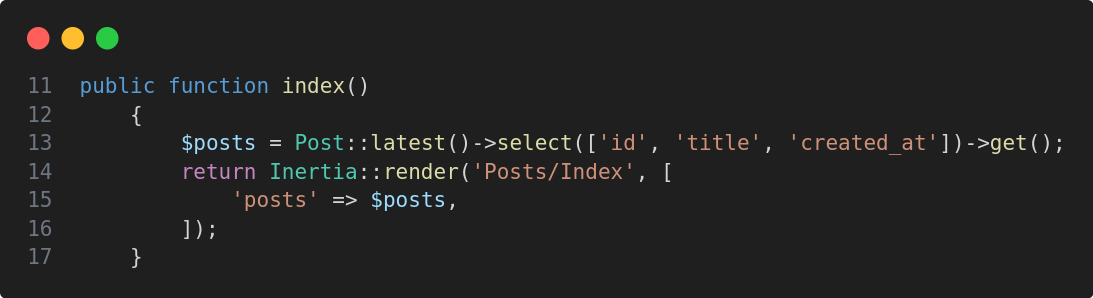
\includegraphics[width=0.4\textwidth]{figures-C1/postscontroller_index.png}
\end{wrapfigure}
Avec cet exemple simple, on comprend vite à quel point il est simple d'interagir avec la \db{} par l'intermédiaire des \models{}. Nos posts sont stockés sous forme d'un array d'objets \php{}, contenant les champs que nous avons spécifiés dans la \migration{}. 

\SaveVerb{post_index}|Index.jsx|
\begin{wrapfigure}[15]{r}{0.581\textwidth}
    \vspace{-0.5cm}
    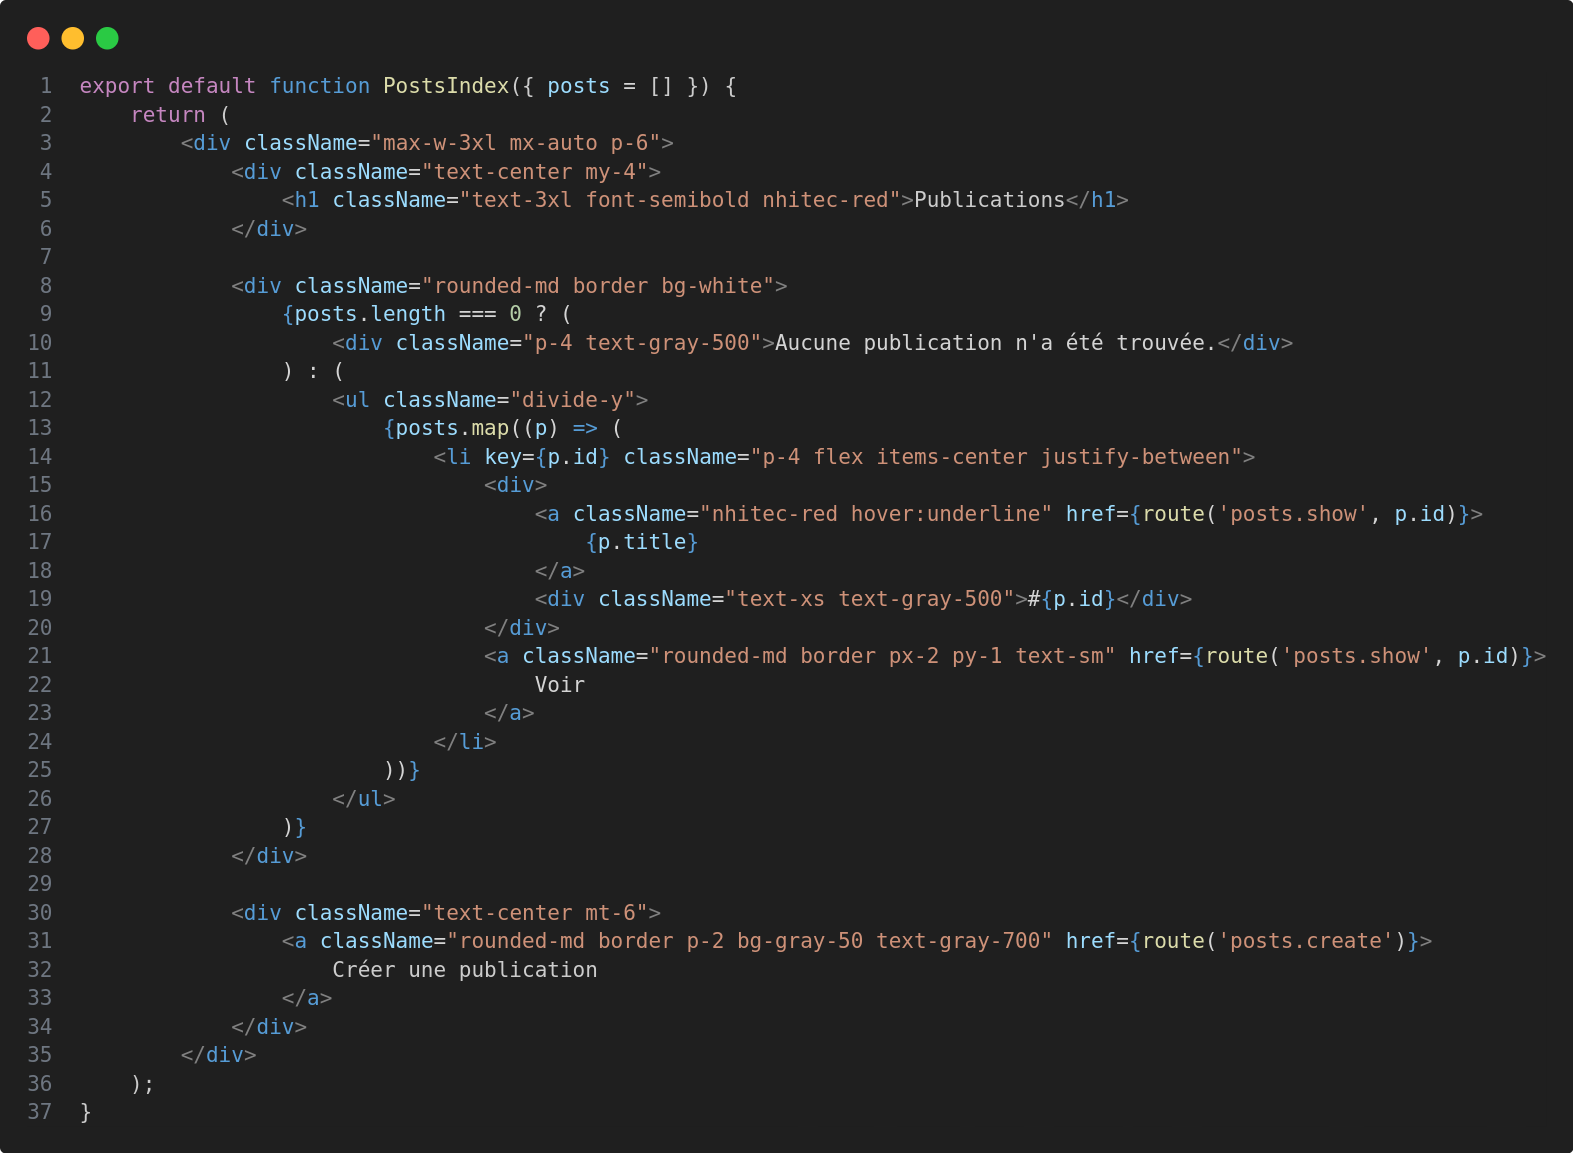
\includegraphics[width=0.581\textwidth]{figures-C1/posts_index.png}
    \caption{\protect\UseVerb{post_index}\label{fig:post_index}}
\end{wrapfigure}
Ensuite, nous allons créer un nouveau dossier \verb|Posts| dans  \\ \verb|resources/js/Pages| et ajouter un fichier dedans appelé \\ \verb|Index.jsx|. Il ne reste ``plus qu'à'' le remplir avec le contenu de la \textsc{Figure~\ref{fig:post_index}}.

Ici, tout est déjà connu mis à part le \verb|posts.length === 0 ? (X) : (Y)|,  \\ qui vérifie s'il y a un post : si non, il affiche X sinon Y \footnote{Il s'agit d'un opérateur ternaire, comme en C, permettant de faire un \texttt{if...else} en une seule ligne.}. Ensuite, il y a le \verb|"."| permettant d'accéder aux différents champs des objets que sont nos \verb|$post|.

Enfin, il ne nous reste plus qu'à ajouter un bouton à notre navbar \footnote{Dans Layouts/AppLayout.jsx (juste de rien pour ça).} afin d'accéder à cette page.

\begin{figure}[!h]
    \centering
    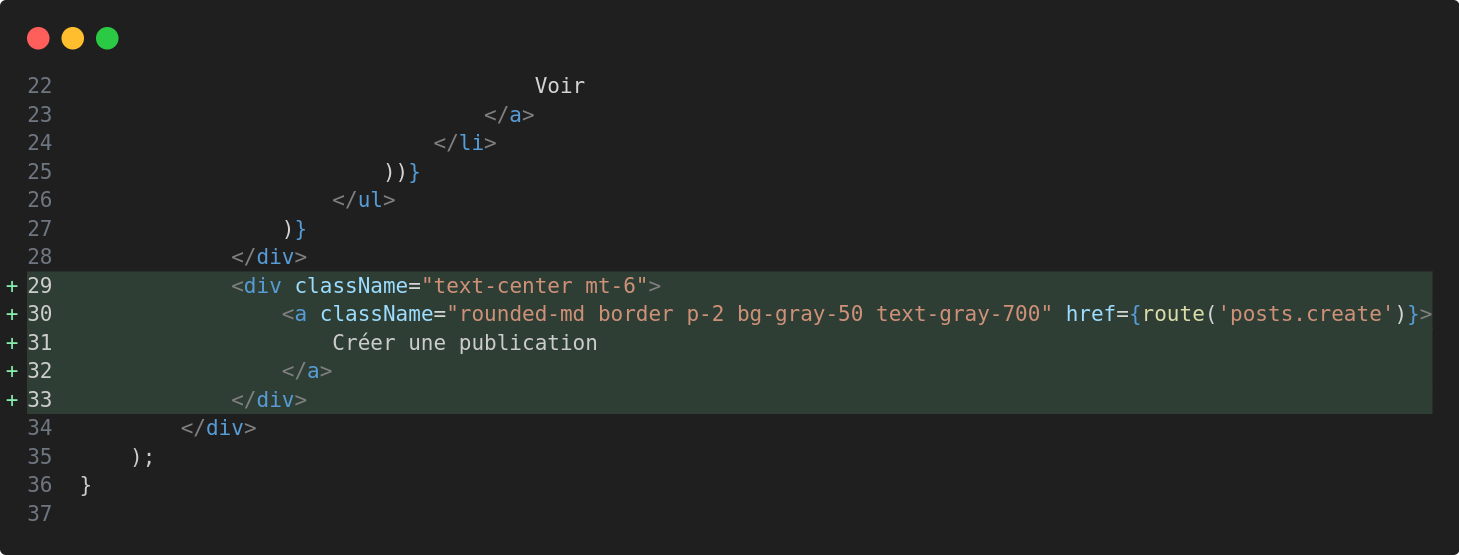
\includegraphics[width=0.75\textwidth]{figures-C1/posts_index_add_create.png}
\end{figure}

\subsubsubsection{show}\label{sec:post_show}

Même chose que pour la page précédente, il faut remplir la fonction \verb|show()|.

\begin{wrapfigure}[3]{r}{0.4\textwidth}
    \vspace{-0.75cm}
    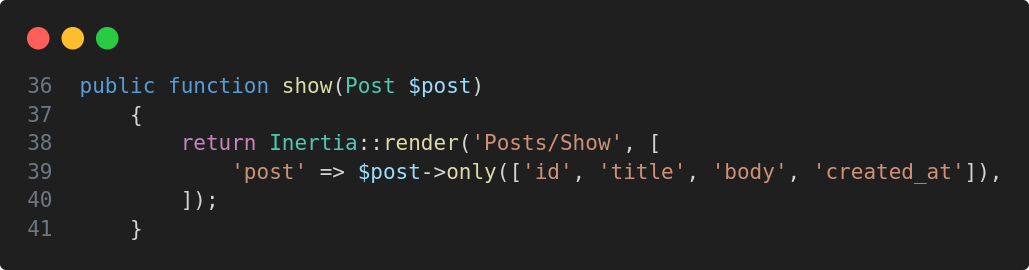
\includegraphics[width=0.4\textwidth]{figures-C1/postscontroller_show.png}
\end{wrapfigure}
Ici, nous utilisons ce que j'ai expliqué en dessous de la \textsc{Figure~\ref{fig:post_route}}. La fonction \verb|show()| prend en argument \verb|$post|. Bah oui, ce qui est logique car pour afficher un post en particulier, il faut donner à \laravel le \texttt{\$post} en question. 

Enfin, la page correspondante peut être créée au nom et emplacement \texttt{resources/js/Pages/Posts/Show.jsx}

\begin{figure}[!h]
    \centering
    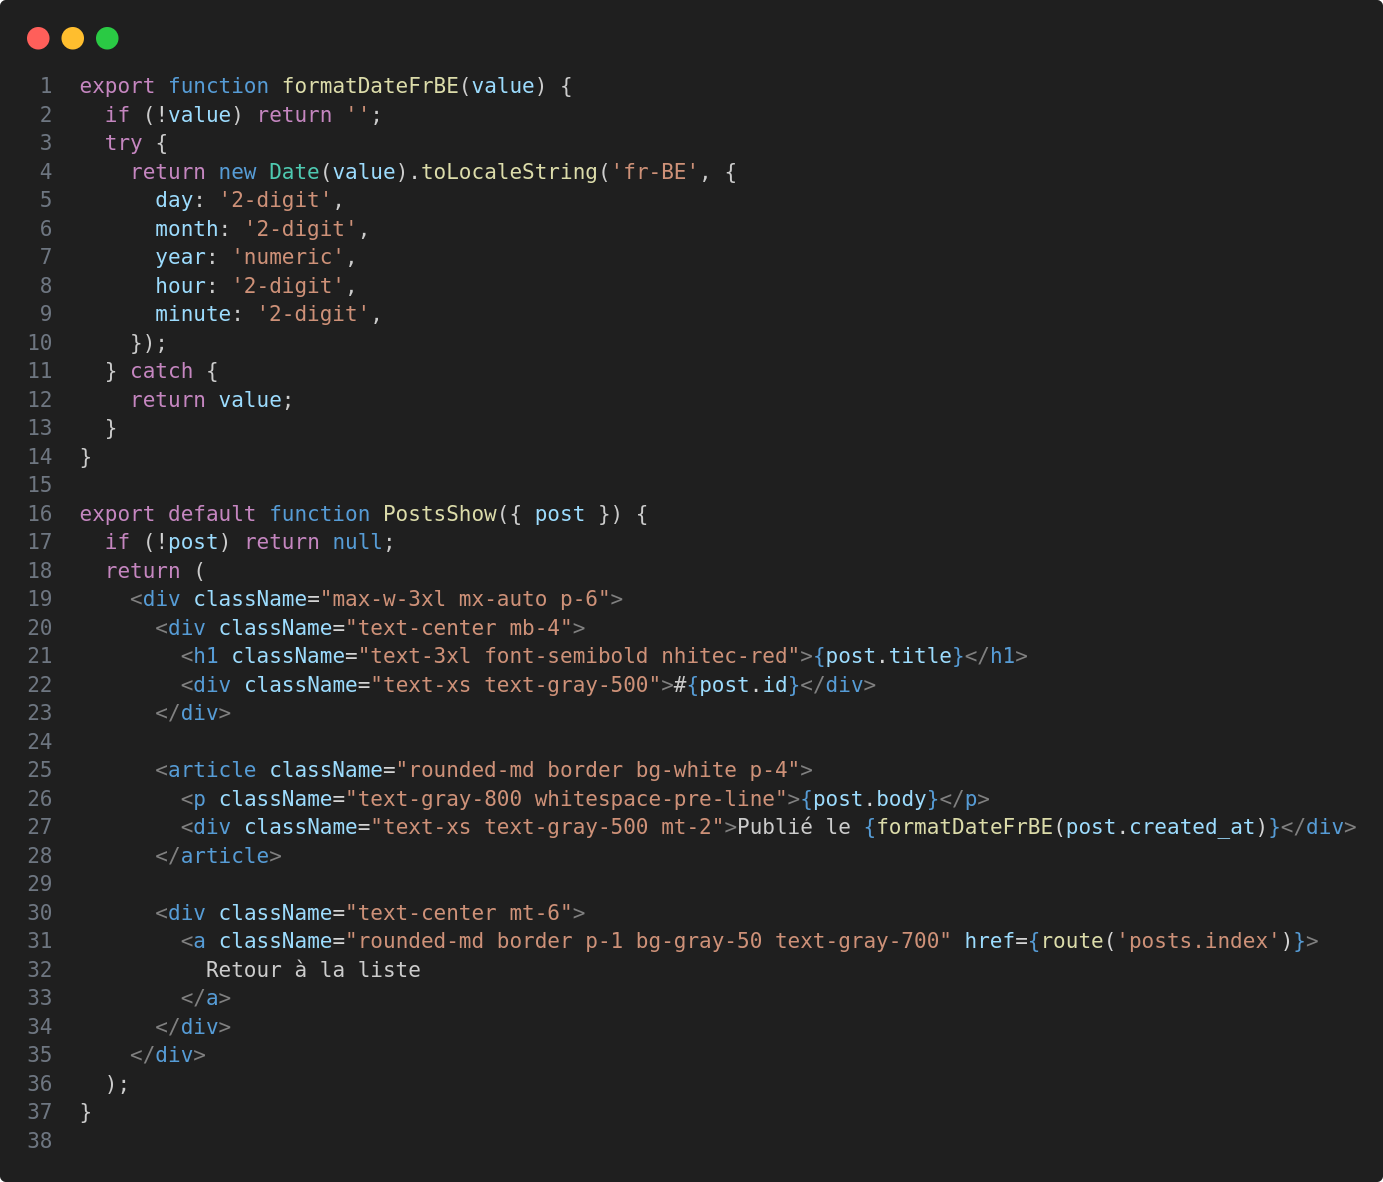
\includegraphics[width=0.75\textwidth]{figures-C1/posts_show.png}
\end{figure}

Ici, on a créé une fonction \texttt{formatDateFrBE()} qui permet d'afficher la date au format belge au lieu du format US.

Hormis ceci, R.A.S. en termes de nouveautés donc nous pouvons maintenant passer à la création de posts!

\subsubsubsection{create}

Cette partie est plus intéressante car elle va amener un nouveau concept, les \forms{}. Jusque ici, nous n'avons jamais eu à rentrer nous-mêmes des données et à les envoyer à notre site pour qu'il fasse des choses avec, c'est exactement à cela que servent les \forms{}.

\begin{wrapfigure}[5]{r}{0.4\textwidth}
    \vspace{-0.5cm}
    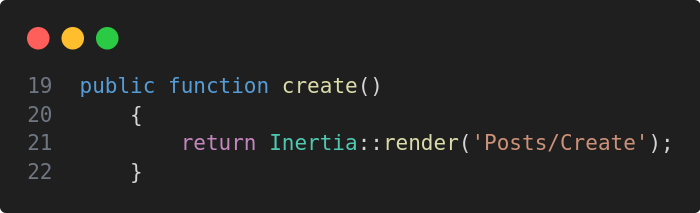
\includegraphics[width=0.4\textwidth]{figures-C1/postscontroller_create.png}
\end{wrapfigure}
Tout d'abord, remplissons la méthode \verb|create()| du \texttt{controller} et créons le fichier \\ \verb|resources/posts/create.jsx| comme nous en avons maintenant l'habitude.

Maintenant, il faut remplir la page:

\begin{figure}[!h]
    \centering
    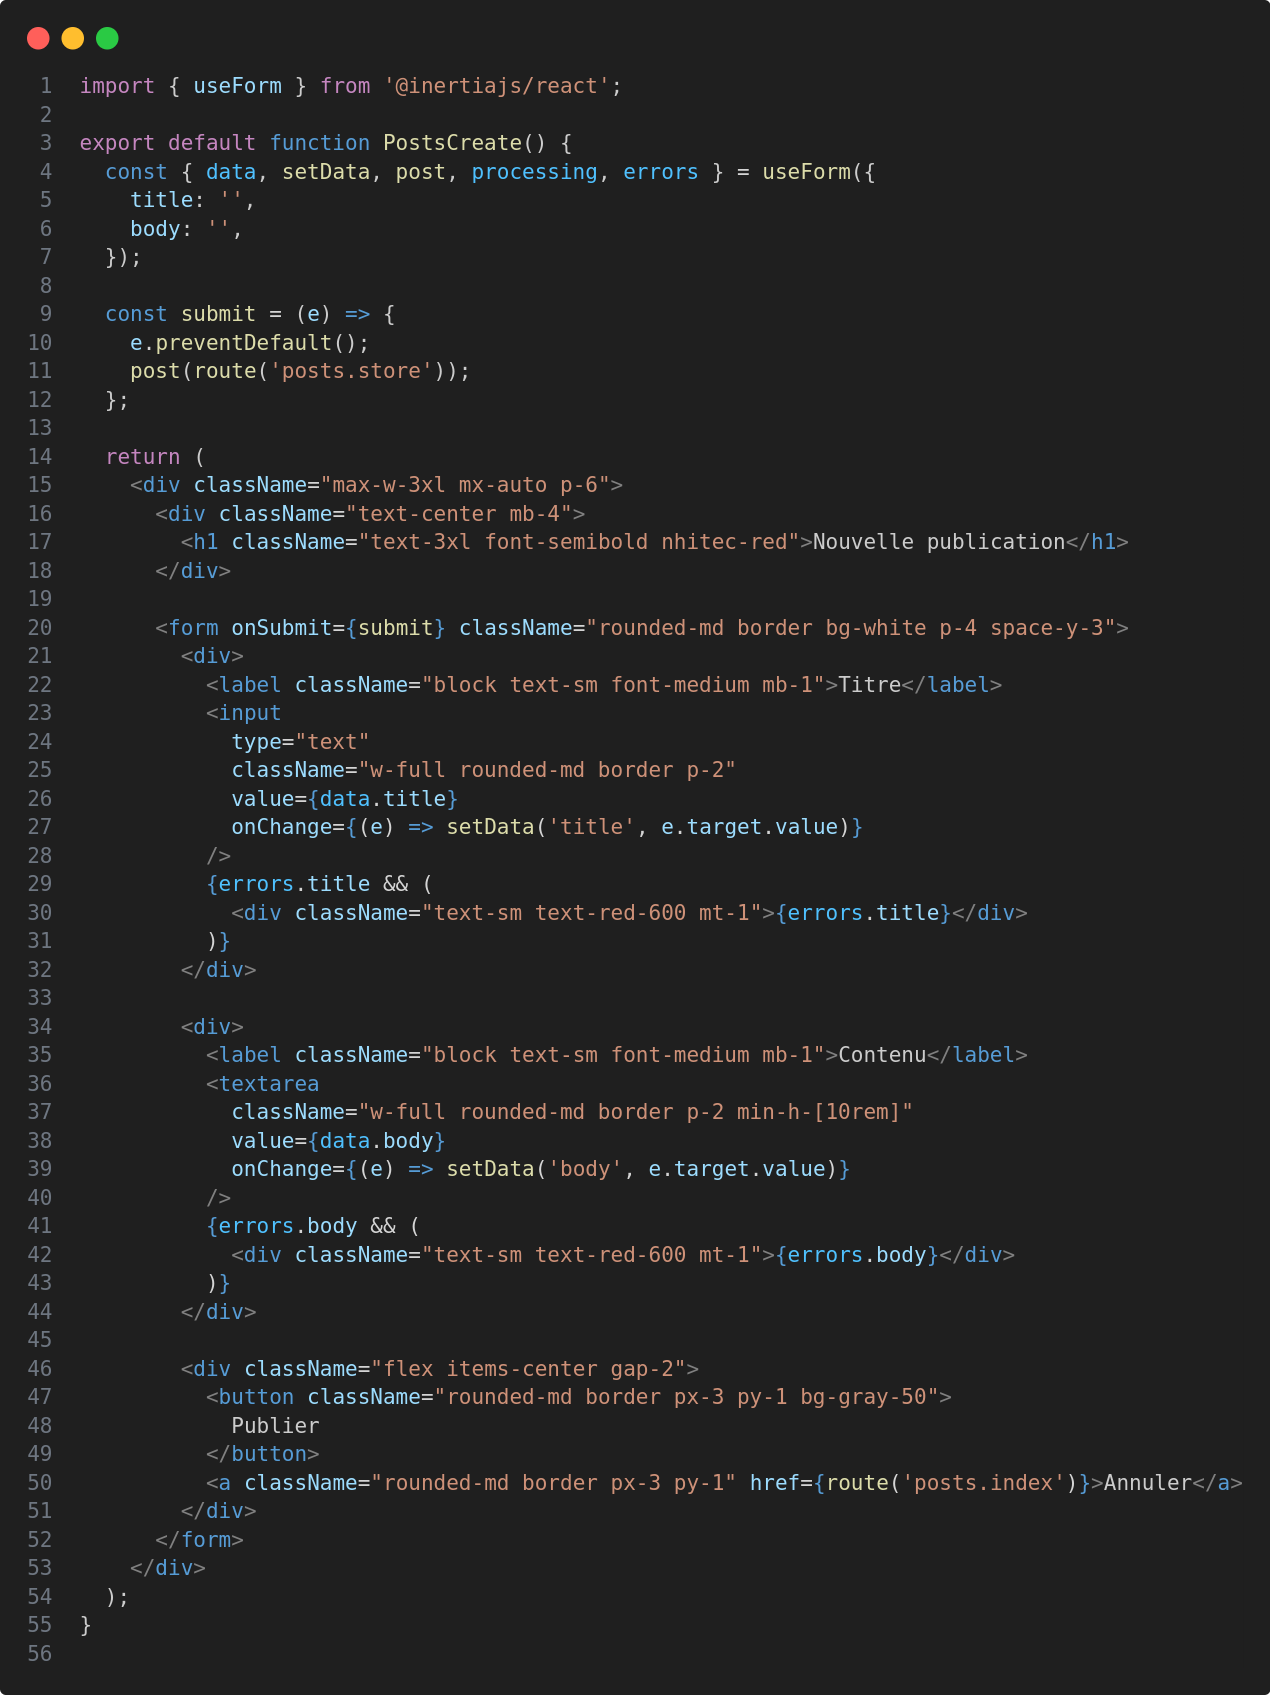
\includegraphics[width=0.8\textwidth]{figures-C1/posts_create.png}
\end{figure}
Ici, il y a pas mal de nouveautés. On voit, en effet, apparaître trois nouveaux tags \html:

\begin{enumerate}
    \item \verb|<form>| : Ce bloc regroupe les champs du formulaire. L'envoi est contrôlé par la fonction passée à \verb|onSubmit|. Dans l'exemple, \verb|submit| empêche le rechargement de la page (\verb|e.preventDefault();|) puis envoie les données via \verb|post(route('posts.store'))|. La fonction \verb|post| provient du hook \verb|useForm| et \verb|route('posts.store')| génère l'URL de la route backend.
    
    \item \verb|<label>| : Sert à afficher un intitulé lisible pour l'utilisateur. Placé juste avant le champ auquel il se rapporte. Pour renforcer l'accessibilité, on pourrait ajouter un attribut \verb|htmlFor| (et un \verb|id| correspondant sur le champ).
    
    \item \verb|<input type="text">| : Champ de saisie contrôlé pour le titre. La valeur affichée provient de l'état (\verb|value={data.title}|). Chaque frappe déclenche \verb|onChange| qui met à jour l'état via \verb|setData('title', e.target.value)| \footnote{Au cas où, le \texttt{e} c'est juste pour pas écrire \texttt{event} au complet, voilà voilà.}. L'affichage conditionnel d'un message d'erreur se fait avec \verb|errors.title|.
    
    \item \verb|<textarea>| : Champ de texte multi-lignes pour le contenu. Il est également contrôlé : \verb|value={data.body}| et mise à jour via \verb|setData('body', e.target.value)|. Le message d'erreur associé utilise \verb|errors.body|.
\end{enumerate}

Bon, ce fût beaucoup (trop) de bla-bla, mais on va (enfin) pouvoir passer à la suite! Promis, les trois dernières méthodes seront bien plus simples. Mais avant cela, n'oubliez pas d'ajouter un bouton sur la page \texttt{Posts/Index.jsx} pour accéder à cette page:

\begin{figure}[!h]
    \centering
    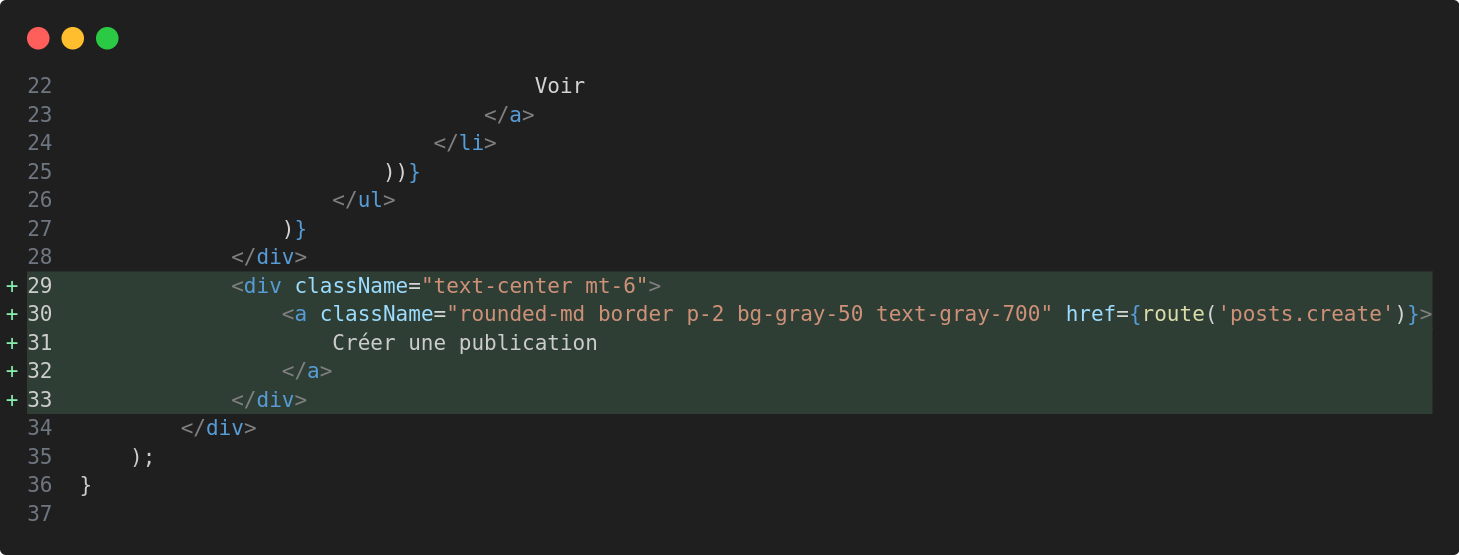
\includegraphics[width=0.75\textwidth]{figures-C1/posts_index_add_create.png}
    \caption{Ajout du bouton "Créer une publication" dans \texttt{Index.jsx }}
\end{figure}

\newpage

\subsubsubsection{store}\label{sec:posts_store}

On a vu à la section précédente que les données du \form{} étaient envoyées à la route \verb|'posts.store'|, or cette \route{} redirige vers cette fonction! C'est donc ici que nous allons stocker le post nouvellement créé.

Tout d'abord, nous allons vérifier si les 2 champs \verb|titre| et \verb|message| ont bien été remplis (s'ils doivent être remplis, ils sont requis $\Rightarrow$ \verb|required|). Pour cela, on utilise la fonction \verb|validate()| de \laravel\footnote{Plus d'informations ainsi que la liste des règles de \texttt{validation} \href{https://laravel.com/docs/12.x/validation#quick-writing-the-validation-logic}{ici}.}. Si la \texttt{validation} rate, l'utilisateur est renvoyé à la page précédente et si elle réussit, alors on continue.

\begin{wrapfigure}[8]{r}{0.5\textwidth}
    \vspace{-0.5cm}
    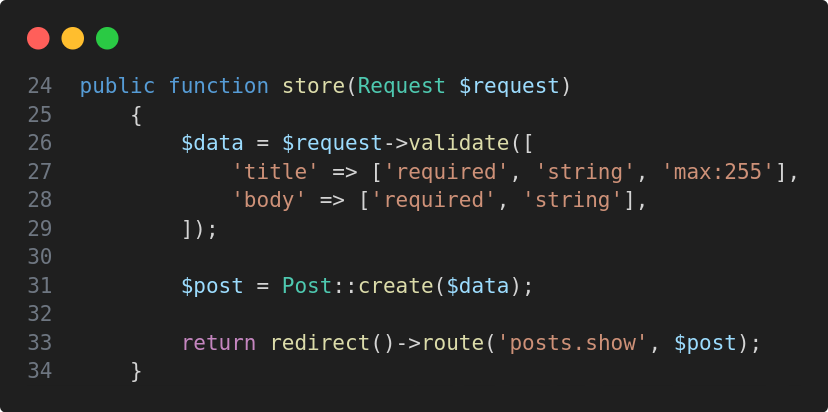
\includegraphics[width=0.5\textwidth]{figures-C1/postscontroller_store.png}
    \caption{Méthode \texttt{store()}}
\end{wrapfigure}
L'étape suivante est de créer un nouveau post, via son \model{}. Ensuite, on remplit ses champs avec les valeurs obtenues dans le \form{} et on le sauvegarde dans la base de données. Enfin, il ne reste plus qu'à envoyer l'utilisateur quelque part (la liste des posts) et le tour est joué!\footnote{La variable \verb|'success'| sera utilisée dans la \texttt{Section~\ref{sec:messages}}.} Plus qu'à rajouter les fonctionnalités de modification et de suppression et puis nous en aurons terminé.

\vspace{1.5cm}
\subsubsubsection{edit}

Pour l'édition, c'est plutôt simple. Tout d'abord, remplissons la méthode du \controller{}:
\vspace{1cm}

\begin{figure}[!h]
    \centering
    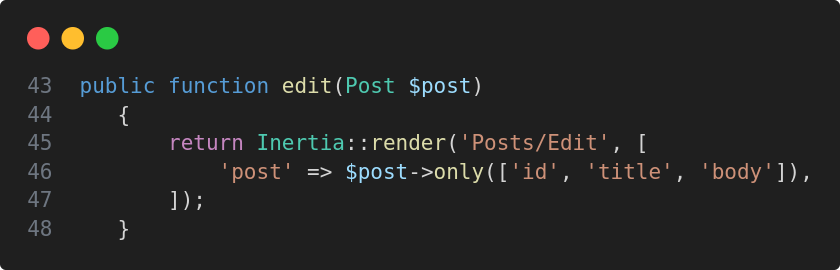
\includegraphics[width=0.8\linewidth]{figures-C1/postscontroller_edit.png}
    \caption{Méthode \texttt{edit}}
    \label{fig:posts-methode-edit}
\end{figure}
\newpage
Ensuite, créons la page dédiée:
\begin{figure}[!h]
    \centering
    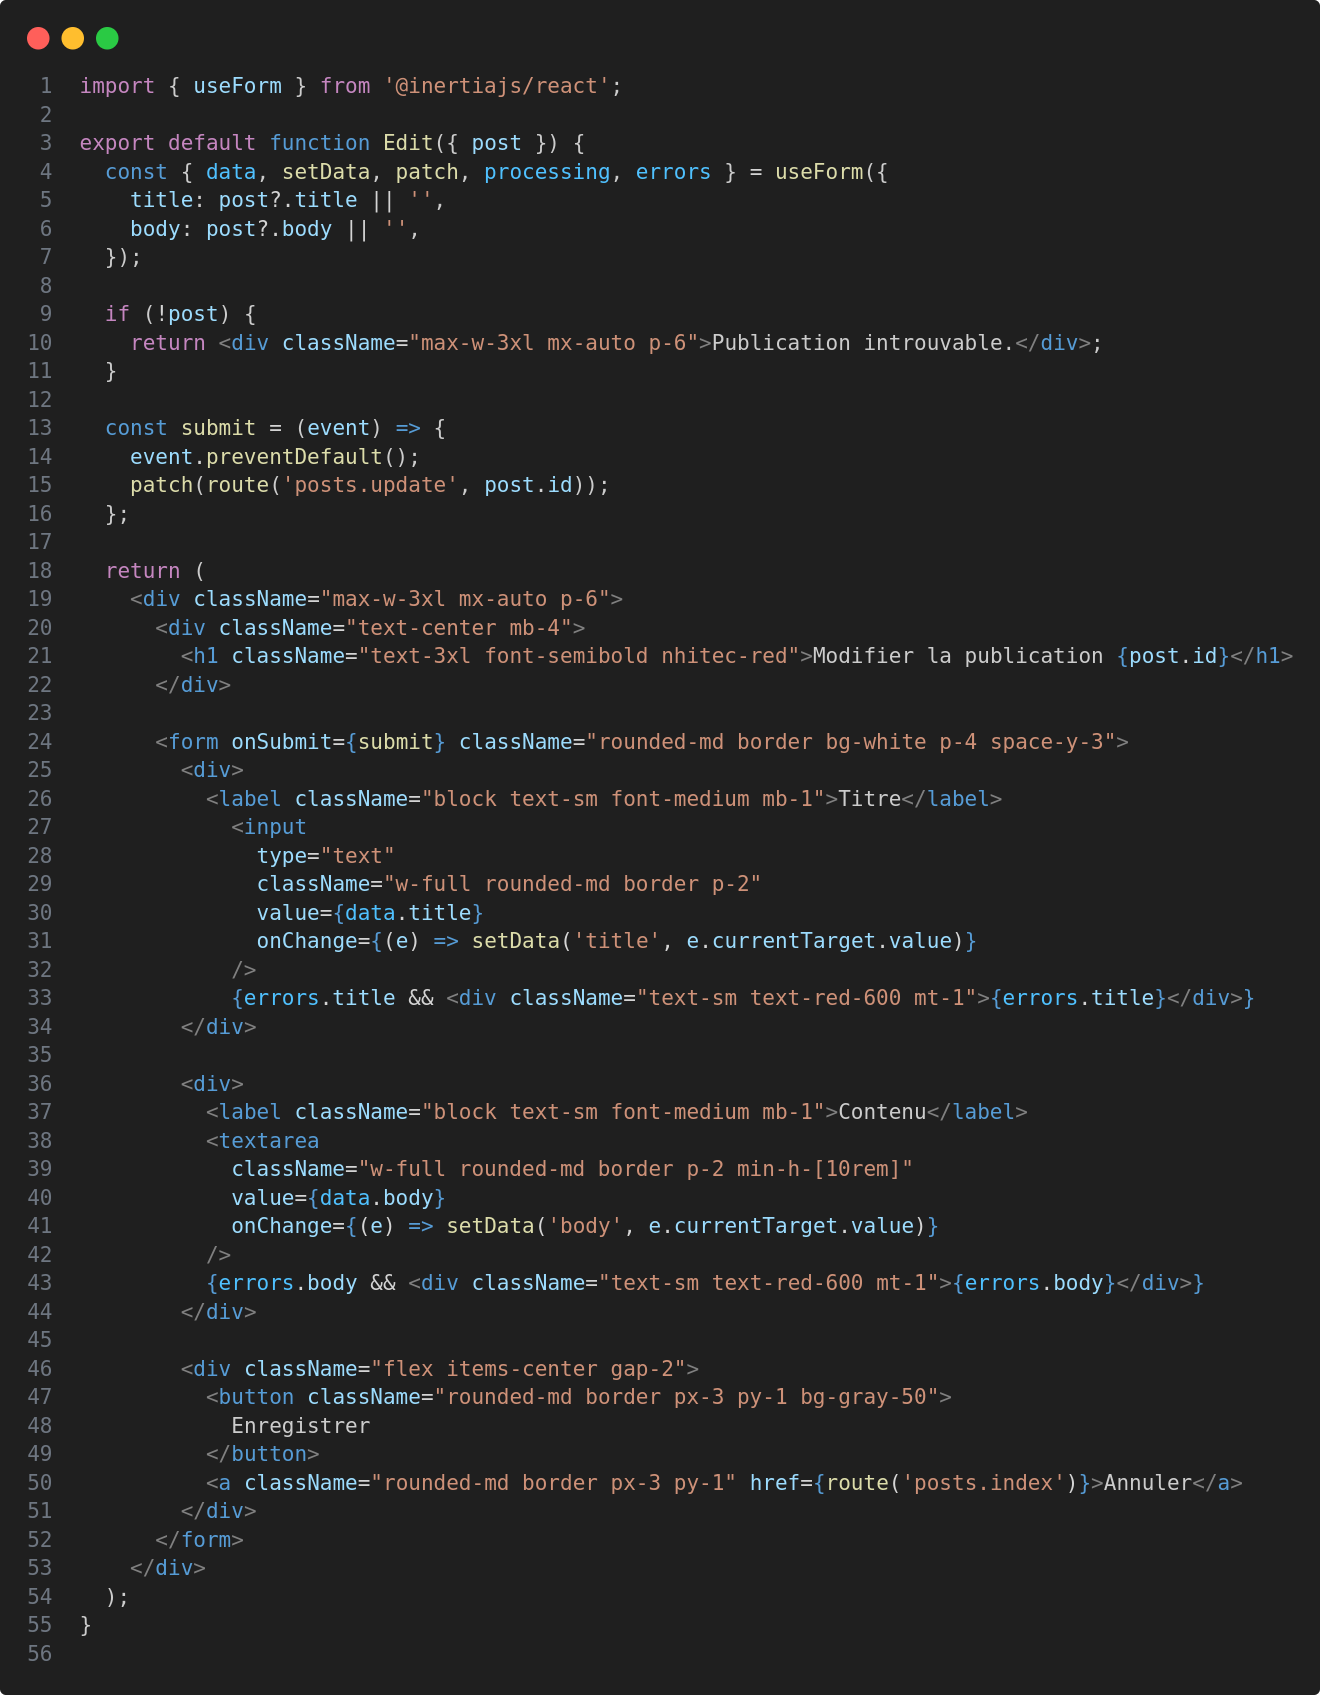
\includegraphics[width=0.75\textwidth]{figures-C1/posts_edit.png}
    \caption{\texttt{Posts/Edit.jsx}}
\end{figure}

Remarquez qu'il n'y a presque aucune différence avec la page de création de post, et c'est bien normal: on peut l'utiliser quasi à l'identique à condition de mettre les valeurs du post dans les bons champs lorsque l'on accède à la page. Une différence est néanmoins à noter, la présence du \verb|patch()|, ligne 15. Cette méthode permet de remplacer une donnée par une autre (notre post à modifier).

\subsubsubsection{update}\label{sec:posts_update}

\begin{wrapfigure}[11]{r}{0.65\textwidth}
    \vspace{-0.5cm}
    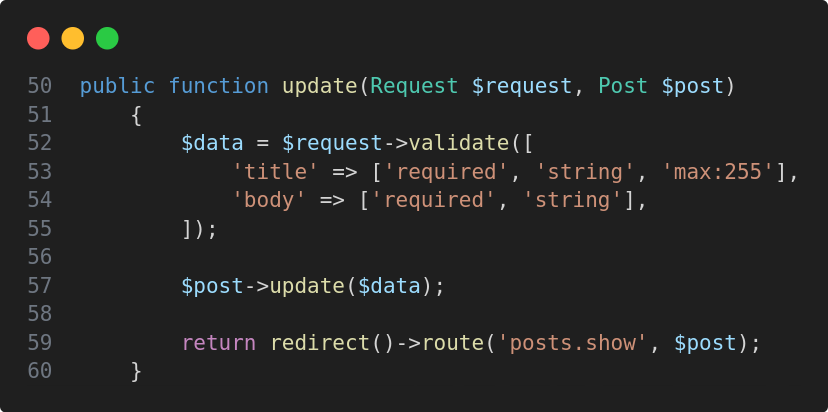
\includegraphics[width=0.65\textwidth]{figures-C1/postscontroller_update.png}
    \caption{Méthode \texttt{update}}
\end{wrapfigure}
Lorsque le \form{} est envoyé, il faut bien sûr enregistrer le post dans notre \db{}. La route \verb|'posts.update'| nous envoit donc vers la méthode \verb|update()| que vous pouvez remplir comme ci-contre. Notez que ici aussi, la démarche est la même que pour la création de post (et c'est logique), mis à part qu'on cherche le post à modifier au lieu d'en créer un nouveau.

\subsubsubsection{destroy}\label{sec:posts_delete}

Enfin, la suppression de post. Tout d'abord, ajoutons deux boutons dans \verb|Posts/Index.jsx|, un qui permet d'accéder à notre page de modification d'un post, et un autre qui permettra de le supprimer (\textsc{Figure~\ref{fig:post_delete_blade}}).

\begin{wrapfigure}[10]{r}{0.65\textwidth}
    \vspace{-0.5cm}
    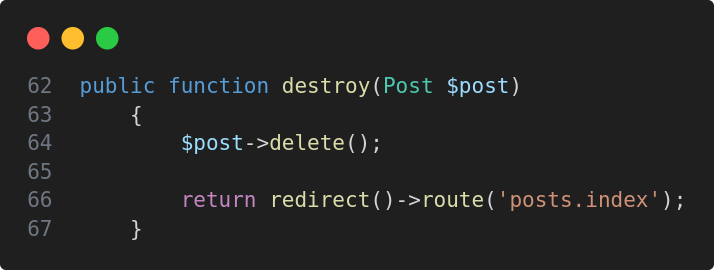
\includegraphics[width=0.65\textwidth]{figures-C1/postscontroller_destroy.png}
    \caption{Méthode \texttt{destroy}}
\end{wrapfigure}
Ensuite, remplissons la méthode du \controller{}. La mécanique est ici triviale, il suffit de sélectionner le post que l'on souhaite et ensuite de le supprimer.

\begin{figure}
    \centering
    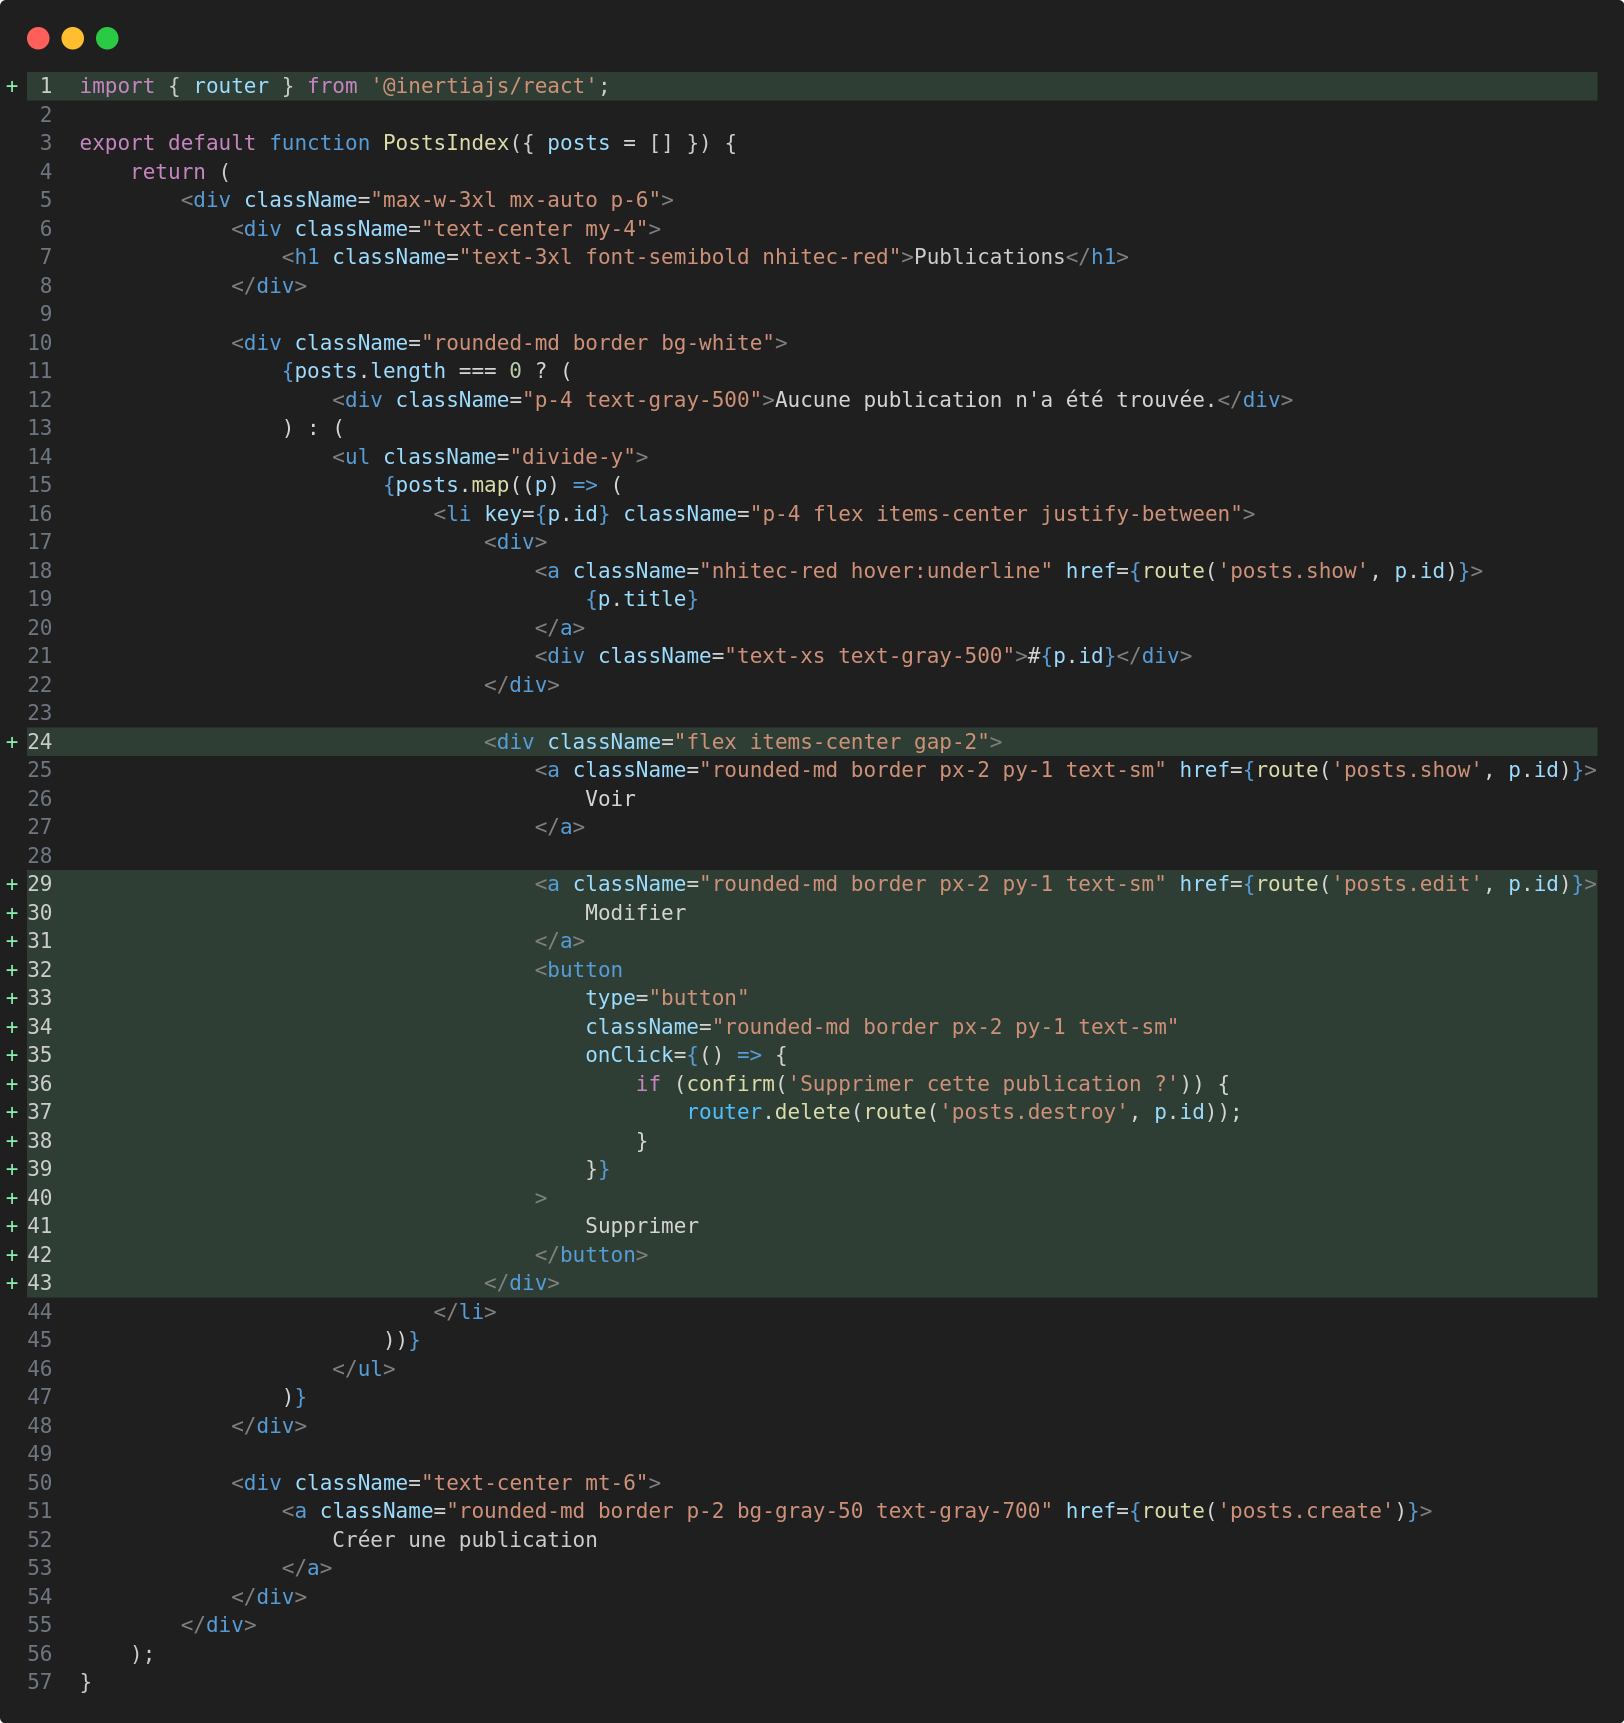
\includegraphics[width=\textwidth]{figures-C1/posts_index_add_edit_delete.png}
    \caption{Ajout des boutons "Modifier" et "Supprimer" dans \texttt{Index.jsx}
    \label{fig:post_delete_blade}}
\end{figure}

Et voilà! Nous avons désormais un système (simple) de création et gestion de posts! Évidemment, nous pourrions rajouter énormément de fonctionnalités (commentaires, auteurs, images, \ldots). Nous explorerons certaines de ces options dans de futures sections, pour cette introduction, c'est déjà plus que suffisant.

A titre d'indication, voici le résultat auquel vous devriez arriver si tout fonctionne correctement:

\begin{figure}[!h]
    \begin{subfigure}[c]{0.55\textwidth}
        \fbox{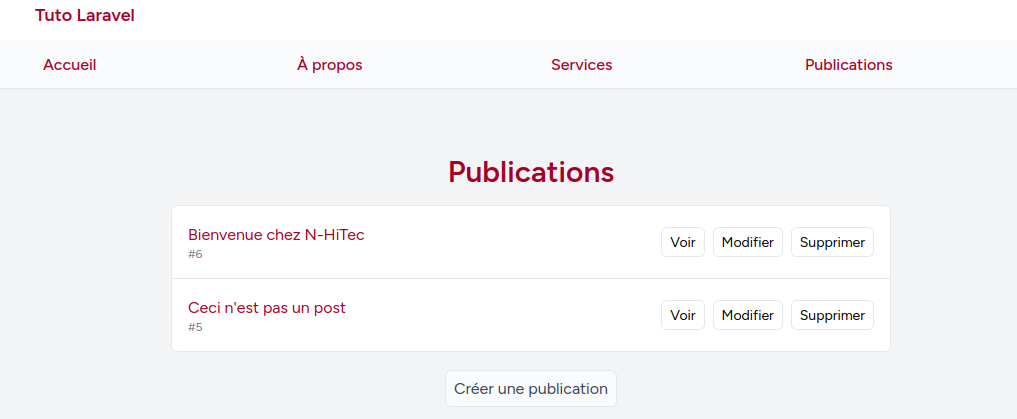
\includegraphics[width=\textwidth]{figures-C1/localhost_posts.png}}
    \end{subfigure}\hfill
    \begin{subfigure}[c]{0.40\textwidth}
        \caption{\url{http://localhost/posts}} 
    \end{subfigure}
    \begin{subfigure}[c]{0.55\textwidth}
        \fbox{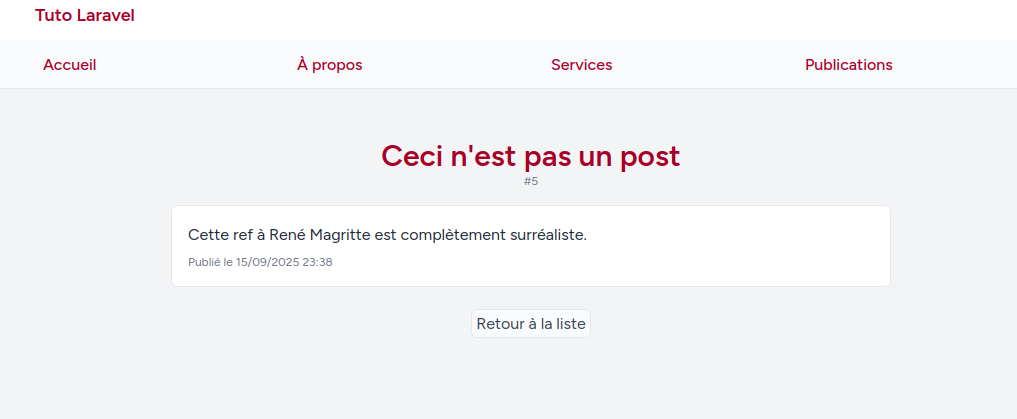
\includegraphics[width=\textwidth]{figures-C1/localhost_show.png}}
    \end{subfigure}\hfill
    \begin{subfigure}[c]{0.40\textwidth}
        \caption{\url{http://localhost/posts/1}} 
    \end{subfigure}
    \begin{subfigure}[c]{0.55\textwidth}
        \fbox{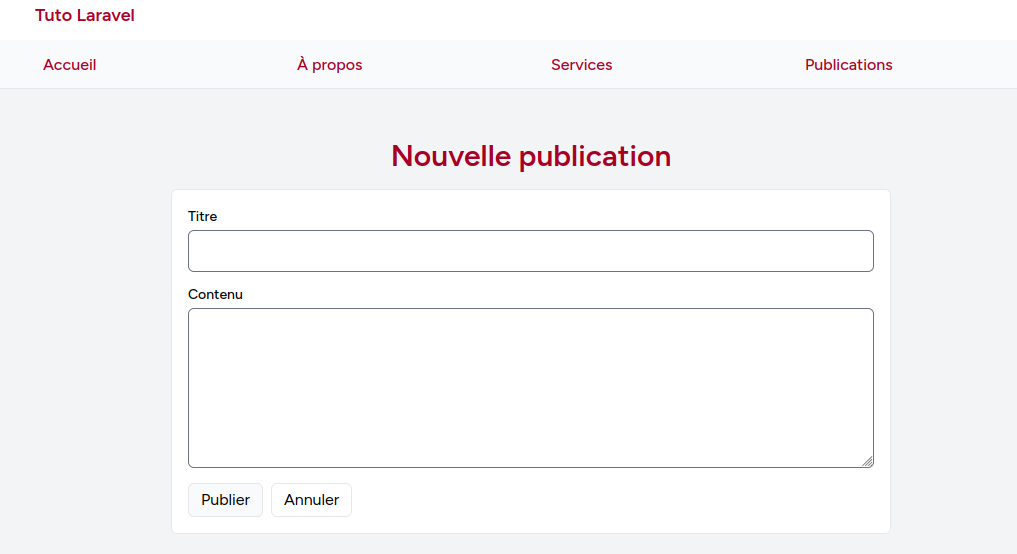
\includegraphics[width=\textwidth]{figures-C1/localhost_create.png}}
    \end{subfigure}\hfill
    \begin{subfigure}[c]{0.40\textwidth}
        \caption{\url{http://localhost/posts/create}} 
    \end{subfigure}
    \begin{subfigure}[c]{0.55\textwidth}
        \fbox{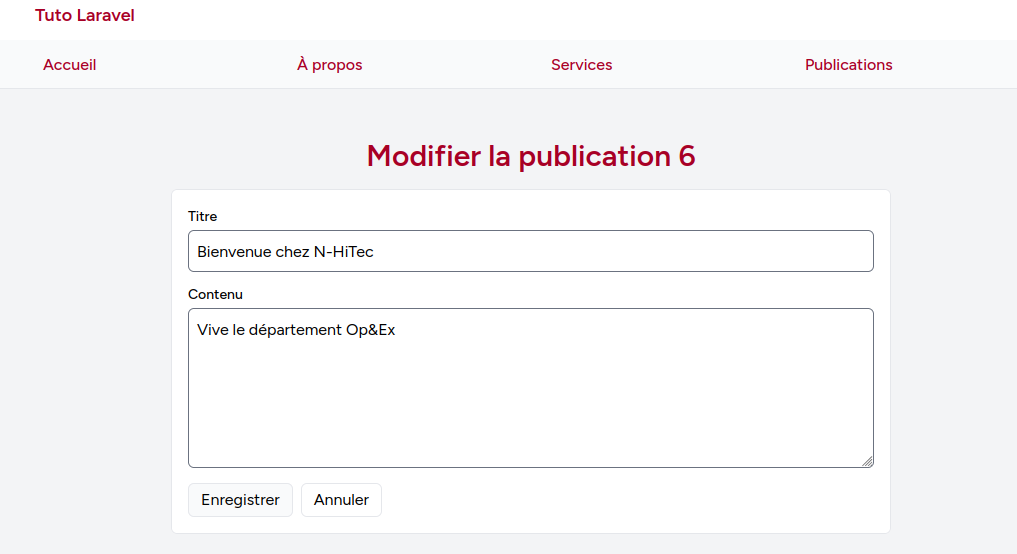
\includegraphics[width=\textwidth]{figures-C1/localhost_edit.png}}
    \end{subfigure}\hfill
    \begin{subfigure}[c]{0.40\textwidth}
        \caption{\url{http://localhost/posts/1/edit}}
    \end{subfigure}
    \caption{Les quatres pages de gestions des posts.}
\end{figure}

\newpage
